\documentclass[11pt,a4paper]{article}

\usepackage[T1]{fontenc}
\usepackage[utf8]{inputenc}
\usepackage{mathptmx}
\usepackage[scaled=0.9]{helvet}
\usepackage[margin=2.3cm]{geometry}
\usepackage{amsmath,amssymb,amsthm,mathtools}
\usepackage{booktabs}
\usepackage{longtable}
\usepackage{tikz}
\usetikzlibrary{arrows.meta,calc,positioning,fit,backgrounds}
\usepackage{microtype}
\usepackage{enumitem}
\usepackage{tcolorbox}
\usepackage[hidelinks]{hyperref}
\usepackage{fancyhdr}
\usepackage{caption}
\usepackage{array}

\tcbuselibrary{skins,breakable}
\captionsetup{font=small,labelfont=bf}

\renewcommand{\contentsname}{Índice}
\renewcommand{\appendixname}{Apéndice}
\renewcommand{\figurename}{Figura}
\renewcommand{\tablename}{Cuadro}

\pagestyle{fancy}
\fancyhf{}
\fancyhead[L]{\footnotesize Protocolo de pruebas · Vision Rover Challenge}
\fancyhead[R]{\footnotesize\thepage}
\renewcommand{\headrulewidth}{0.4pt}

\newcommand{\R}{\mathbb{R}}
\newcommand{\Rot}{\mathbf{R}}
\newcommand{\uu}{\mathbf{u}}
\newcommand{\nn}{\mathbf{n}}
\newcommand{\dd}{\mathbf{d}}
\newcommand{\cc}{\mathbf{c}}
\newcommand{\pp}{\mathbf{p}}
\newcommand{\vv}{\mathbf{v}}
\newcommand{\ww}{\mathbf{w}}
\newcommand{\ee}{\mathbf{e}}
\newcommand{\gv}{\mathbf{g}}
\newcommand{\aaa}{\mathbf{a}}
\newcommand{\NN}{\mathbf{N}}
\newcommand{\atantwo}{\operatorname{atan2}}
\newcommand{\conv}{\operatorname{conv}}
\newcommand{\sgn}{\operatorname{sgn}}
\newcommand{\grados}{^{\circ}}
\newcommand{\MM}[1]{\textsc{m}:\,\ref{#1}}

% --- entorno de prueba -----------------------------------------------------
\newcounter{pruebactr}
\newenvironment{prueba}[2]{%
  \par\medskip\noindent
  \begin{tcolorbox}[enhanced,breakable,colback=white,colframe=black!45,
    boxrule=0.5pt,arc=1pt,left=6pt,right=6pt,top=4pt,bottom=4pt,
    title={\bfseries #1\quad\normalfont #2},
    colbacktitle=black!8,coltitle=black,fonttitle=\bfseries\small]
  \small
}{\end{tcolorbox}\par\medskip}

\newcommand{\campo}[1]{\par\smallskip\noindent\textbf{#1}\quad\ignorespaces}

\begin{document}

\begin{titlepage}
\centering
\vspace*{2cm}
{\Large\scshape Universidad Hispanoamericana}\\[0.2cm]
{\large Ingeniería Mecatrónica}\\[2.2cm]

\rule{\linewidth}{1.2pt}\\[0.4cm]
{\LARGE\bfseries Protocolo de verificación y validación\\[0.18cm]
del modelo matemático}\\[0.4cm]
\rule{\linewidth}{1.2pt}\\[0.8cm]

{\large Especificación de pruebas sin hardware físico:\\
consistencia interna, estimadores geométricos, visión extremo a extremo,\\
capa de planificación y simulación de lazo cerrado}\\[2.2cm]

\begin{tabular}{rl}
\textbf{Autor} & Sebastián Vega Amores\\[0.12cm]
\textbf{Documento verificado} & \textit{Modelo matemático para la detección, localización}\\
 & \textit{y planificación geométrica del transporte de objetos cúbicos}\\[0.12cm]
\textbf{Sistema bajo prueba} & Vision Rover Challenge, protocolo de telemetría v1\\[0.12cm]
\textbf{Fecha} & 2 de septiembre de 2026\\
\end{tabular}

\vfill
{\small Este documento \emph{especifica} las pruebas. Los resultados de su ejecución se
reportan por separado en el informe de resultados.}
\end{titlepage}

\tableofcontents
\newpage

% =========================================================================
\section{Estrategia de verificación}

\subsection{El problema: validar sin tocar el hardware}

Un modelo matemático puede fallar de cuatro maneras distintas, y cada una se
descubre con una clase de prueba diferente. Confundirlas es la razón habitual por
la que un sistema pasa todas las pruebas y falla el día de la competencia.

\begin{table}[htbp]
\centering
\small
\caption{Las cuatro clases de falla y el banco que las revela.}
\begin{tabular}{p{3.3cm}p{5.4cm}p{5.6cm}}
\toprule
Clase de falla & En qué consiste & Cómo se descubre \\
\midrule
\textbf{Error algebraico} & Un signo, una convención invertida, una identidad mal
derivada. El modelo es internamente inconsistente. & Verificando \emph{invariantes}:
propiedades que deben cumplirse para todo valor de entrada. Nivel N0. \\
\addlinespace
\textbf{Error de estimación} & La fórmula es correcta pero el estimador es sesgado,
ineficiente o frágil ante ruido y valores atípicos. & Comparando contra
\emph{verdad conocida} generada analíticamente, con y sin ruido. Nivel N1. \\
\addlinespace
\textbf{Error de modelo} & Las hipótesis no describen el sistema real: el modelo es
correcto sobre un mundo que no es este. & Contrastando contra un simulador
\emph{independiente} del modelo, que renderiza el mundo por otro camino. Nivel N2. \\
\addlinespace
\textbf{Error de composición} & Cada pieza funciona aislada, pero encadenadas se
degradan, se realimentan o entran en modos no previstos. & Ejercitando el
\emph{lazo cerrado} completo bajo perturbación. Niveles N3 y N4. \\
\bottomrule
\end{tabular}
\label{tab:clases}
\end{table}

La consecuencia práctica es que \textbf{no existe una única prueba que valide el
modelo}. Se necesita una jerarquía, y cada nivel solo tiene sentido si el anterior
pasó: medir la precisión de un estimador cuya álgebra tiene un signo invertido es
medir cuidadosamente algo equivocado.

\subsection{La jerarquía de niveles}

\begin{figure}[htbp]
\centering
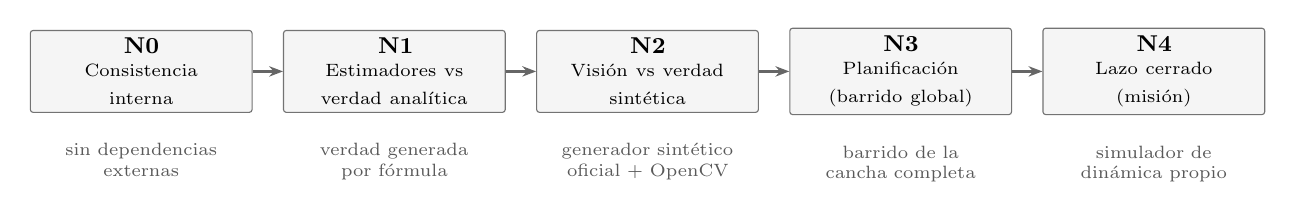
\begin{tikzpicture}[node distance=0pt,font=\small,scale=0.92,transform shape]
\tikzset{
  nivel/.style={draw=black!55,fill=black!4,rounded corners=1pt,
    minimum height=1.05cm,text width=2.85cm,align=center,inner sep=3pt},
  fl/.style={-{Stealth[length=5pt]},black!60,thick}
}
\node[nivel] (n0) {\textbf{N0}\\[1pt]\scriptsize Consistencia\\\scriptsize interna};
\node[nivel,right=0.42cm of n0] (n1) {\textbf{N1}\\[1pt]\scriptsize Estimadores vs\\\scriptsize verdad analítica};
\node[nivel,right=0.42cm of n1] (n2) {\textbf{N2}\\[1pt]\scriptsize Visión vs verdad\\\scriptsize sintética};
\node[nivel,right=0.42cm of n2] (n3) {\textbf{N3}\\[1pt]\scriptsize Planificación\\\scriptsize (barrido global)};
\node[nivel,right=0.42cm of n3] (n4) {\textbf{N4}\\[1pt]\scriptsize Lazo cerrado\\\scriptsize (misión)};
\draw[fl] (n0) -- (n1); \draw[fl] (n1) -- (n2);
\draw[fl] (n2) -- (n3); \draw[fl] (n3) -- (n4);
\node[below=0.3cm of n0,font=\scriptsize,text width=2.9cm,align=center,black!65]
  {sin dependencias\\externas};
\node[below=0.3cm of n1,font=\scriptsize,text width=2.9cm,align=center,black!65]
  {verdad generada\\por fórmula};
\node[below=0.3cm of n2,font=\scriptsize,text width=2.9cm,align=center,black!65]
  {generador sintético\\oficial + OpenCV};
\node[below=0.3cm of n3,font=\scriptsize,text width=2.9cm,align=center,black!65]
  {barrido de la\\cancha completa};
\node[below=0.3cm of n4,font=\scriptsize,text width=2.9cm,align=center,black!65]
  {simulador de\\dinámica propio};
\end{tikzpicture}
\caption{Jerarquía de verificación. Cada nivel presupone que el anterior pasó.
La independencia de la fuente de verdad crece hacia la derecha: N1 se valida contra
la misma fórmula que implementa, N2 contra un renderizador que no comparte código con
el modelo.}
\label{fig:niveles}
\end{figure}

\begin{tcolorbox}[colback=black!3,colframe=black!50,boxrule=0.5pt,arc=1pt]
\textbf{El principio que ordena la jerarquía: independencia de la fuente de verdad.}
Una prueba solo vale lo que vale su referencia. Comparar un estimador contra la misma
ecuación que implementa detecta errores de programación, no de modelo. Por eso N2 es
cualitativamente más fuerte que N1: el generador sintético construye la imagen por
proyección directa de un cubo tridimensional, sin usar en ningún momento el modelo de
silueta ni las fórmulas de estimación. Si ambos coinciden, la coincidencia es
informativa.
\end{tcolorbox}

\subsection{Qué banco de pruebas existe y qué falta}

El repositorio oficial ya provee dos bancos, y le falta un tercero.

\begin{table}[htbp]
\centering
\small
\caption{Infraestructura de prueba disponible en el repositorio.}
\begin{tabular}{p{3.6cm}p{4.3cm}p{6.4cm}}
\toprule
Componente & Qué provee & Limitación para nuestro propósito \\
\midrule
\texttt{sources/gene\-rador\_sintetico.py} &
Renderiza imágenes del tablero con marcadores, rovers y cubos, \textbf{conociendo la
verdad} de lo que dibujó: pose de cámara, paralaje, oclusión por orden de dibujo. &
Ninguna para N2: es exactamente la referencia independiente que hace falta. No
simula dinámica ni acepta comandos. \\
\addlinespace
\texttt{tools/verificar\_*.py} &
Cuatro verificaciones contra esa verdad: geometría, rovers, cubos, seguimiento. &
Miden \textbf{posición} del cubo, nunca su \textbf{ángulo}, aunque el detector lo
calcula. El ángulo queda sin verificar. \\
\addlinespace
\texttt{contrato/mock\_pu\-blisher.py} &
Emite telemetría v1 con ruido, oclusiones, pérdidas de detección y cubos que se
mueven al ser empujados. & \textbf{No acepta comandos.} Los rovers se mueven solos.
No hay manera de cerrar el lazo percepción$\,\to\,$decisión$\,\to\,$acción. \\
\addlinespace
\textit{(ausente)} & --- &
\textbf{Falta un simulador de dinámica} que consuma las decisiones del planificador,
mueva el rover con cinemática diferencial, resuelva el contacto con el cubo y
realimente telemetría. Es lo que construye el nivel N4. \\
\bottomrule
\end{tabular}
\label{tab:infra}
\end{table}

\subsection{Brecha detectada en el simulador oficial}
\label{sec:brecha}

\begin{tcolorbox}[colback=black!5,colframe=black!65,boxrule=0.7pt,arc=1pt]
\textbf{Hallazgo H-01 --- El modelo de contacto del simulador oficial no es
geométricamente compatible con el rover físico.}

\medskip
\texttt{config\_simulador.json} declara \texttt{radio\_empuje\_celdas} $=1{,}5$ y
\texttt{radio\_oclusion\_celdas} $=2{,}0$, ambos medidos entre el \textbf{centro del
rover} y el \textbf{centro del cubo}. En unidades métricas: $30\ \mathrm{mm}$ y
$40\ \mathrm{mm}$.

Pero la distancia real entre centros en el instante de contacto es
\[
  \varrho_{\mathrm{cont}} = \frac{L}{2}\big(|\cos\Delta|+|\sin\Delta|\big) + \frac{\Lambda}{2}
  \in [\,100{,}0;\ 112{,}4\,]\ \mathrm{mm} = [\,5{,}00;\ 5{,}62\,]\ \text{celdas},
\]
es decir entre \textbf{3,3 y 3,7 veces} el radio de empuje declarado. Con cuerpos
rígidos de $120\times140\ \mathrm{mm}$ y cubos de $60\ \mathrm{mm}$, que el centro del
rover llegue a $30\ \mathrm{mm}$ del centro del cubo es geométricamente imposible: el
rover ya habría atravesado el cubo.

\medskip
\textbf{Consecuencias.}
\begin{enumerate}[label=(\alph*),leftmargin=2em,itemsep=1pt]
\item Un planificador calibrado contra el simulador aprenderá a \emph{acercarse
      demasiado} y en la cancha empujará el cubo antes de llegar a su punto de puesta,
      o lo desviará lateralmente.
\item El simulador \textbf{nunca ocluye un cubo durante un empuje legítimo}
      ($5{,}0 > 2{,}0$ celdas), justo el caso que el sistema de visión real reporta
      como el más frecuente y que degrada la detección de $1{,}05$ a
      $4{,}88\ \mathrm{mm}$. La lógica de manejo de \texttt{age\_ms} queda sin ejercitar
      donde más importa.
\item El empuje del simulador es \emph{isótropo} (depende solo de la distancia entre
      centros), mientras que el real es \emph{direccional}: solo empuja lo que está
      delante de las paletas.
\end{enumerate}

\medskip
\textbf{Tratamiento adoptado.} No se modifica el simulador oficial: es la referencia
normativa del contrato y su valor está en emitir telemetría con el formato correcto.
Se construye el simulador de dinámica del nivel N4 con la geometría de contacto
correcta, y se documenta la discrepancia como riesgo de transferencia. Se recomienda
elevar el punto a la organización.
\end{tcolorbox}

\subsection{Criterio general de aceptación}

Cada prueba declara su criterio. Se adoptan tres tipos:

\begin{description}[leftmargin=2.4em,style=nextline,font=\normalfont\itshape]
\item[Exactitud numérica.] El resultado debe coincidir con la verdad salvo error de
  redondeo: $|\hat x - x| \le \varepsilon_{\mathrm{maq}}$ con
  $\varepsilon_{\mathrm{maq}} = 10^{-9}$ en las unidades de la magnitud. Se aplica a
  identidades algebraicas y estimadores sin ruido.
\item[Cota física.] El resultado debe respetar un umbral con significado físico
  (milímetros, grados). Se aplica a estimadores con ruido y a la cadena de visión.
\item[Propiedad universal.] Una relación debe cumplirse para \emph{todo} punto de un
  barrido o de un muestreo aleatorio, sin excepción. Un solo contraejemplo reprueba.
  Se aplica a invariantes, cotas y condiciones de factibilidad.
\end{description}

\subsection{Notación de las fichas de prueba}

Cada prueba se especifica con cuatro campos: \textbf{Hipótesis} (qué afirmación del
modelo pone a prueba), \textbf{Método} (cómo se genera la evidencia),
\textbf{Criterio} (qué constituye aprobar) y \textbf{Justificación} (por qué esta
prueba y no otra). Los identificadores \textsc{m}: remiten a teoremas y
ecuaciones del documento del modelo matemático.

% =========================================================================
\section{Nivel N0 --- Consistencia interna del modelo}

Propósito: descartar errores algebraicos y de convención antes de medir nada. Todas
las pruebas de este nivel son \emph{propiedades universales} verificadas sobre
barridos densos, sin ninguna dependencia externa.

\begin{prueba}{N0.1}{Ortogonalidad del operador de rotación}
\campo{Hipótesis} $\Rot(\theta)^{\mathsf T}\Rot(\theta) = I$ y $\det\Rot(\theta)=1$
para todo $\theta$ (\textsc{m}:\,proposición~2.6a--b).
\campo{Método} Barrido $\theta \in [-720\grados, 720\grados]$ con paso $0{,}1\grados$
(14\,401 evaluaciones).
\campo{Criterio} Exactitud numérica: $\|\Rot^{\mathsf T}\Rot - I\|_\infty \le 10^{-12}$
y $|\det\Rot - 1| \le 10^{-12}$ en todo el barrido.
\campo{Justificación} Es la propiedad de la que dependen todas las demás: si $\Rot$ no
es una isometría, las distancias del modelo no son distancias. El barrido excede
$[0,360\grados)$ a propósito, para verificar que no hay dependencia de rama en la
implementación.
\end{prueba}

\begin{prueba}{N0.2}{Homomorfismo de rotaciones}
\campo{Hipótesis} $\Rot(\alpha)\Rot(\beta) = \Rot(\alpha+\beta)$ (\textsc{m}:\,proposición~2.6a).
\campo{Método} Producto cartesiano de $\alpha,\beta$ sobre una malla de $2\grados$ en
$[0\grados,360\grados)$ ($32\,400$ pares).
\campo{Criterio} Propiedad universal, exactitud numérica $10^{-12}$.
\campo{Justificación} Es lo que autoriza a componer giros sin acumular error de
convención, y lo que sostiene la recursión de $90\grados$ del teorema \textsc{m}:\,teorema~4.6.
\end{prueba}

\begin{prueba}{N0.3}{Acción sobre versores y recuperación del argumento}
\campo{Hipótesis} $\Rot(\theta)\uu(\varphi) = \uu(\theta+\varphi)$ (\textsc{m}:\,proposición~2.6c) y
$\atantwo(-u_y, u_x) \equiv \alpha \pmod{360\grados}$ para $\uu = \uu(\alpha)$
(apéndice A del modelo).
\campo{Método} Malla de $1\grados$ en ambos argumentos.
\campo{Criterio} Propiedad universal, $10^{-9}$ en grados tras normalizar por
$\rho_{360}$.
\campo{Justificación} La segunda mitad es la operación inversa que usan \emph{todos}
los estimadores de ángulo del modelo (B1, B2, B3). Un signo mal puesto aquí produce
ángulos espejados que igual parecen razonables.
\end{prueba}

\begin{prueba}{N0.4}{Forma cerrada de la rotación de $90\grados$}
\campo{Hipótesis} $\Rot(90\grados)(\delta_x,\delta_y)^{\mathsf T} =
(\delta_y, -\delta_x)^{\mathsf T}$ (\textsc{m}:\,proposición~2.6d).
\campo{Método} $10^5$ vectores aleatorios de módulo en $[10^{-6}, 10^{3}]$.
\campo{Criterio} Exactitud numérica $10^{-12}$.
\campo{Justificación} Esta identidad es la que permite generar los cuatro vértices sin
trigonometría. Si difiere aunque sea en el último bit del cálculo matricial, la
optimización deja de ser equivalente y hay que saberlo.
\end{prueba}

\begin{prueba}{N0.5}{Convención de pantalla (fila descendente)}
\campo{Hipótesis} $\uu(0\grados) = (1,0)$ apunta hacia \texttt{col} creciente y
$\uu(90\grados) = (0,-1)$ apunta hacia \texttt{row} \emph{decreciente}, es decir hacia
arriba en la imagen.
\campo{Método} Evaluación directa en $\{0,90,180,270\}\grados$ y verificación del signo
de cada componente.
\campo{Criterio} Coincidencia exacta con los cuatro versores canónicos y con la
convención declarada en la sección 4 del contrato oficial.
\campo{Justificación} Es la convención más fácil de invertir y la más costosa de
descubrir tarde: un rover que gira al revés parece un problema de motores. Se ancla
contra el texto del contrato, no contra el modelo, para que la prueba sea
independiente.
\end{prueba}

\begin{prueba}{N0.6}{Diferencia angular con signo}
\campo{Hipótesis} $\delta(\alpha,\beta) \in (-180\grados, 180\grados]$;
$\delta(\alpha,\beta) \equiv \alpha-\beta \pmod{360\grados}$;
$\delta(\alpha,\beta) = -\delta(\beta,\alpha)$ salvo en el borde $180\grados$
(\textsc{m}:\,ec.~(4)).
\campo{Método} Malla de $0{,}5\grados$ en ambos argumentos sobre
$[-360\grados, 720\grados]$, más los casos frontera $(359{,}9;\,0{,}1)$,
$(0;\,180)$, $(180;\,0)$, $(0;\,0)$.
\campo{Criterio} Propiedad universal en rango y congruencia; el caso
$\delta(359{,}9\grados,\ 0{,}1\grados)$ debe dar $-0{,}2\grados$ y no $359{,}8\grados$.
\campo{Justificación} El cierre del círculo es la fuente clásica de fallas
intermitentes: el error aparece solo cuando el rover cruza el norte. Se prueba
explícitamente el cruce.
\end{prueba}

\begin{prueba}{N0.7}{Distancia angular de periodo $P$}
\campo{Hipótesis} $\rho_P(\alpha,\beta) \in [0, P/2]$, es simétrica, se anula si y solo
si $\alpha\equiv\beta \pmod P$, y $\rho_{90}$ acota por $45\grados$ (\textsc{m}:\,ec.~(5)).
\campo{Método} Barrido para $P\in\{90\grados, 360\grados\}$, malla de $0{,}25\grados$,
más verificación contra la definición por minimización explícita
$\min_{k}|\alpha-\beta+kP|$ con $k \in \{-4,\dots,4\}$.
\campo{Criterio} Propiedad universal; coincidencia con la minimización explícita a
$10^{-9}$.
\campo{Justificación} Comparar la forma cerrada contra la definición por minimización
es la única manera de verificar que la fórmula \emph{es} lo que dice ser, y no una
aproximación que funciona en el rango que se probó.
\end{prueba}

\begin{prueba}{N0.8}{Identidades del marco fila-descendente}
\campo{Hipótesis} Las siete identidades del apéndice A del modelo:
$\uu(\alpha)\cdot\uu(\beta) = \cos(\alpha-\beta)$;
$\uu(\alpha)\wedge\uu(\beta) = -\sin(\beta-\alpha)$;
$\uu(\alpha)+\uu(\alpha+90\grados) = \sqrt2\,\uu(\alpha+45\grados)$;
$\uu(\alpha+90\grados)-\uu(\alpha) = \sqrt2\,\uu(\alpha+135\grados)$;
$\partial_\alpha \uu(\alpha) = \uu(\alpha+90\grados)$.
\campo{Método} Malla de $1\grados$; la derivada por diferencias centradas con
$h=10^{-6}$ rad.
\campo{Criterio} Exactitud $10^{-10}$ para las algebraicas, $10^{-6}$ para la derivada
numérica.
\campo{Justificación} Estas identidades se usan implícitamente en las demostraciones de
\textsc{m}:\,proposición~4.7 y \textsc{m}:\,teorema~4.9. Verificarlas por separado localiza el error si
alguna de esas pruebas falla.
\end{prueba}

% =========================================================================
\section{Nivel N1 --- Estimadores geométricos contra verdad analítica}

Propósito: verificar que los estimadores de pose recuperan exactamente lo que se les
dio, y que su degradación bajo ruido es la predicha. La verdad se genera por fórmula
directa; el estimador debe invertirla.

\subsection{El modelo del cuadrado}

\begin{prueba}{N1.1}{Parametrización vertical: propiedades métricas}
\campo{Hipótesis} Los cuatro puntos de \textsc{m}:\,ec.~(17) forman un cuadrado de lado $L$:
las cuatro aristas miden $L$, las dos diagonales miden $L\sqrt2$, el área vale $L^2$,
y el centroide de los cuatro vértices es $\cc$.
\campo{Método} Producto cartesiano de $\theta \in [0\grados,360\grados)$ paso
$0{,}5\grados$ y $\cc$ sobre una malla de $5\times5$ posiciones en la cancha; área por
la fórmula del polígono (\textit{shoelace}).
\campo{Criterio} Exactitud numérica $10^{-9}$ relativa, en las cuatro propiedades
simultáneamente.
\campo{Justificación} Comprobar el lado no basta: un rombo también tiene cuatro lados
iguales. La combinación lado $+$ diagonal $+$ área identifica el cuadrado sin
ambigüedad. El barrido en $\theta$ recorre las cuatro ramas de $\atantwo$.
\end{prueba}

\begin{prueba}{N1.2}{Equivalencia de la recursión de $90\grados$}
\campo{Hipótesis} Generar los vértices por \textsc{m}:\,ec.~(17) (trigonométrica) y por
\textsc{m}:\,ec.~(20) (intercambio y cambio de signo) produce el mismo conjunto ordenado.
\campo{Método} Mismo barrido de N1.1.
\campo{Criterio} Exactitud numérica $10^{-12}$ vértice a vértice.
\campo{Justificación} La recursión es la forma que se implementará en tiempo real. La
prueba certifica que la optimización no cambió el resultado, que es exactamente la
clase de regresión que nadie mira hasta que falla.
\end{prueba}

\begin{prueba}{N1.3}{Invariancia bajo el grupo $C_4$}
\campo{Hipótesis} $S(\cc,\theta) = S(\cc,\theta+90\grados k)$ como \emph{conjunto de
puntos}, para todo $k\in\mathbb Z$ (\textsc{m}:\,proposición~4.2).
\campo{Método} Para $\theta$ en malla de $1\grados$ y $k \in \{-2,\dots,2\}$, comparar
los conjuntos de vértices ordenándolos canónicamente (por ángulo respecto de $\cc$).
\campo{Criterio} Propiedad universal, coincidencia a $10^{-9}$.
\campo{Justificación} Justifica reducir el espacio de búsqueda a $[0\grados,90\grados)$.
Si la invariancia fallara, el barrido grueso del detector estaría explorando un
cociente equivocado.
\end{prueba}

\begin{prueba}{N1.4}{Aristas, puntos medios y normales exteriores}
\campo{Hipótesis} \textsc{m}:\,proposición~4.7: $\|\ee_k\| = L$;
$\|\mathbf m_k - \cc\| = L/2$; $\ee_k\cdot\nn_k = 0$; y $\nn_k$ apunta hacia afuera,
es decir $\cc + (L/2+\epsilon)\nn_k \notin S$ para $\epsilon>0$.
\campo{Método} Barrido de $\theta$ paso $0{,}5\grados$, $k\in\{0,1,2,3\}$; la
exterioridad por prueba de punto en polígono con $\epsilon = 10^{-3}L$.
\campo{Criterio} Propiedad universal.
\campo{Justificación} El sentido de la normal decide de qué lado se coloca el rover.
Una normal invertida produce un planificador que intenta empujar desde adentro del
cubo, falla que en simulación se manifiesta como \emph{el rover atraviesa el cubo} y
es fácil de atribuir erróneamente al motor de colisiones.
\end{prueba}

\subsection{Los estimadores de la familia B}

\begin{prueba}{N1.5}{Estimador B1 --- vértice de referencia y centro}
\campo{Hipótesis} \textsc{m}:\,proposición~5.8 recupera $\theta \bmod 90\grados$ exactamente.
\campo{Método} Barrido $\theta \in [0\grados, 90\grados)$ paso $0{,}01\grados$
(9\,000 casos), $\times$ los cuatro vértices de referencia $k\in\{0,1,2,3\}$,
$\times$ 5 posiciones de $\cc$.
\campo{Criterio} $\rho_{90}(\hat\theta,\theta) \le 10^{-9}$ grados en todos los casos.
\campo{Justificación} Es el estimador que corresponde directamente a la propuesta de
trabajo (un vértice de referencia y rotaciones sucesivas). Probarlo con los cuatro
vértices verifica que la reducción módulo $90\grados$ absorbe correctamente la
elección de referencia.
\end{prueba}

\begin{prueba}{N1.6}{Estimador B2 --- arista}
\campo{Hipótesis} \textsc{m}:\,teorema~5.9: $\hat\theta = \atantwo(-e_y,e_x) \bmod 90\grados$
recupera $\theta$ desde \emph{cualquiera} de las cuatro aristas.
\campo{Método} Mismo barrido de N1.5, evaluando las cuatro aristas y ambos sentidos de
recorrido ($\vv_a\to\vv_b$ y $\vv_b\to\vv_a$).
\campo{Criterio} $\rho_{90}(\hat\theta,\theta)\le 10^{-9}$ para las ocho combinaciones.
\campo{Justificación} La invariancia al \emph{sentido} de la arista no es obvia y es
operativamente crítica: un extractor de contornos no garantiza el orden de recorrido.
Si dependiera del sentido, el estimador daría $\theta$ o $\theta+45\grados$ según cómo
haya salido el contorno.
\end{prueba}

\begin{prueba}{N1.7}{Estimador B2 --- desambiguación del signo de la normal}
\campo{Hipótesis} El criterio \textsc{m}:\,ec.~(34) elige el semiplano correcto, para
cualquier posición del punto testigo $\boldsymbol\mu$ dentro del cubo.
\campo{Método} Para $\theta$ en malla de $2\grados$ y cada arista, tomar como testigo:
(i) el centro exacto, (ii) $200$ puntos aleatorios uniformes en el interior del
cuadrado, (iii) el centroide de la silueta con paralaje (caso realista, que está
\emph{fuera} del cuadrado, desplazado hacia afuera del nadir).
\campo{Criterio} El centro recuperado debe coincidir con el verdadero a $10^{-9}$ en
los casos (i) y (ii). El caso (iii) se reporta por separado: se documenta la fracción
de aciertos y la geometría en que falla.
\campo{Justificación} \textbf{Esta prueba busca un cabo suelto específico.} El teorema
supone un testigo interior, pero el testigo disponible en la práctica ---el centroide
de la mancha--- está desplazado por el paralaje y puede caer fuera del cuadrado. Hay
que saber si el criterio sobrevive a eso o si necesita un testigo distinto.
\end{prueba}

\begin{prueba}{N1.8}{Estimador B3 --- diagonal}
\campo{Hipótesis} El par de vértices opuestos determina $\cc$ como punto medio y
$\theta$ salvo $45\grados$ módulo $90\grados$.
\campo{Método} Barrido de N1.5 con ambos pares diagonales.
\campo{Criterio} Exactitud $10^{-9}$ en $\cc$ y en $\rho_{90}(\hat\theta,\theta)$.
\campo{Justificación} Verifica que el desfase de $45\grados$ está bien aplicado. Es un
error de un solo término que produce un cubo perfectamente rotado $45\grados$, lo que
en el peor caso convierte la anchura mínima en la máxima.
\end{prueba}

\begin{prueba}{N1.9}{Estimador B4 --- Procrustes sin ruido}
\campo{Hipótesis} \textsc{m}:\,teorema~5.11 recupera $(\cc,\theta)$ exactamente cuando los
vértices son exactos, para todo subconjunto $\mathcal K$ de tamaño $\ge 2$.
\campo{Método} Los $11$ subconjuntos de $\{0,1,2,3\}$ con $|\mathcal K|\ge2$,
$\times$ barrido de $\theta$ paso $0{,}5\grados$.
\campo{Criterio} Exactitud $10^{-9}$ en posición y en $\rho_{90}$ del ángulo.
\campo{Justificación} Incluye deliberadamente los subconjuntos \emph{diagonales}
$\{0,2\}$ y $\{1,3\}$, donde los vectores centrados son colineales. Ese es el caso
degenerado: hay que verificar que $(\mathcal A,\mathcal B)\ne(0,0)$ y que la solución
sigue siendo única, o documentar que no lo es.
\end{prueba}

\begin{prueba}{N1.10}{Estimador B4 --- insesgadez y eficiencia bajo ruido}
\campo{Hipótesis} \textsc{m}:\,teorema~5.12: el estimador es insesgado y
$\sigma_{\hat\theta} = \sigma/(\varrho_{\mathrm{ef}}\sqrt n)$.
\campo{Método} Monte Carlo con $50\,000$ realizaciones por configuración, para
$n\in\{2,3,4\}$ y $\sigma \in \{0{,}25;\ 0{,}5;\ 1;\ 2;\ 4\}\ \mathrm{mm}$; se estima
el sesgo (media del error) y la desviación empírica, y se contrasta contra la
predicción.
\campo{Criterio} Sesgo compatible con cero dentro de $3$ errores estándar de la media;
desviación empírica dentro del $5\%$ de la predicción para $\sigma \le 2\ \mathrm{mm}$.
\campo{Justificación} El barrido en $\sigma$ busca el punto donde la aproximación de
primer orden deja de valer. Una cota de Cramér--Rao es asintótica; hay que conocer el
régimen de ruido en que todavía describe la realidad, porque el peor caso medido de la
visión con oclusión ($4{,}88\ \mathrm{mm}$) está cerca del extremo del barrido.
\end{prueba}

\begin{prueba}{N1.11}{Estimador B4 --- ruptura ante un vértice atípico}
\campo{Hipótesis} \textbf{Hipótesis de falla:} el estimador de mínimos cuadrados
\emph{no} es robusto; un solo vértice espurio lo sesga sin cota.
\campo{Método} Con $n=4$ vértices exactos, desplazar uno de ellos una distancia
$d \in [0, 200]\ \mathrm{mm}$ en dirección aleatoria; medir el error resultante en
$\hat\theta$ y $\hat\cc$ en función de $d$.
\campo{Criterio} \textbf{Esta prueba está diseñada para reprobar.} Lo que se exige es
caracterizar la pendiente $\partial \hat\theta/\partial d$ y confirmar que crece sin
saturarse. Si el error saturara, habría robustez no prevista y el modelo estaría
incompleto en el otro sentido.
\campo{Justificación} Un extractor de vértices real producirá falsos positivos (una
esquina del rover, un reflejo). Saber que B4 no los tolera obliga a anteponer una
etapa robusta ---mediana de estimaciones por arista, o \textsc{ransac} sobre
subconjuntos--- y esa conclusión debe salir de una medición, no de una intuición.
\end{prueba}

\subsection{Función soporte, anchura y silueta}

\begin{prueba}{N1.12}{Función soporte: forma cerrada contra máximo explícito}
\campo{Hipótesis} \textsc{m}:\,ec.~(25): $h_S(\varphi)-\cc\cdot\uu(\varphi) =
\tfrac{L}{2}(|\cos\Delta|+|\sin\Delta|)$.
\campo{Método} Para cada par $(\theta,\varphi)$ en malla de $1\grados$, calcular el
soporte por maximización explícita sobre los cuatro vértices y comparar con la fórmula.
\campo{Criterio} Propiedad universal, exactitud $10^{-9}$.
\campo{Justificación} La fórmula cerrada es la que sostiene todo el argumento de
factibilidad del empuje. Verificarla contra el máximo explícito la valida sin suponer
que el máximo se alcanza en un vértice, que es precisamente el paso de la demostración
que podría estar mal aplicado.
\end{prueba}

\begin{prueba}{N1.13}{Cota universal de anchura proyectada}
\campo{Hipótesis} \textsc{m}:\,ec.~(26): $L \le w_S(\varphi) \le L\sqrt2$ para todo
$(\theta,\varphi)$, con los extremos alcanzados en $\Delta \equiv 0$ y
$\Delta \equiv 45\grados \pmod{90\grados}$.
\campo{Método} Malla fina de $0{,}1\grados$ en $\Delta$ ($900$ puntos por período), más
$10^6$ pares aleatorios uniformes.
\campo{Criterio} Propiedad universal para la cota; los extremos deben alcanzarse a
$10^{-9}$ en los ángulos predichos.
\campo{Justificación} Es el resultado del que depende que el empuje sea factible sin
conocer el ángulo. Un solo contraejemplo invalida la conclusión operativa central del
modelo, así que se prueba con densidad muy superior a la habitual.
\end{prueba}

\begin{prueba}{N1.14}{Lema de silueta: conteo de vértices del casco convexo}
\campo{Hipótesis} \textsc{m}:\,lema~4.10: la silueta tiene $6$ vértices con el nadir
exterior a la base y $4$ con el nadir interior.
\campo{Método} Barrido del nadir sobre una malla de $2\ \mathrm{m}\times2\ \mathrm{m}$
alrededor del cubo (paso $25\ \mathrm{mm}$), $\times$ $\theta$ en
$\{0,7{,}5,\dots,82{,}5\}\grados$, $\times$ $\kappa$ para alturas de cámara
$\{1300, 1700, 2100\}\ \mathrm{mm}$. Se incluyen explícitamente los casos con el nadir
sobre una arista y sobre un vértice de la base.
\campo{Criterio} Se reporta el histograma de conteos. El lema se considera confirmado
si los casos de $6$ y $4$ vértices se explican por la posición del nadir, y se
\emph{documentan} las configuraciones degeneradas (nadir sobre arista o vértice) en
lugar de tratarlas como fallas.
\campo{Justificación} El lema afirma «genéricamente seis». Una prueba honesta tiene que
buscar activamente las configuraciones no genéricas y decir cuántas son y dónde están,
en vez de muestrear al azar donde el resultado es cómodo.
\end{prueba}

\subsection{Paralaje}

\begin{prueba}{N1.15}{Paralaje: la corrección es una involución exacta}
\campo{Hipótesis} $\pi^{-1}(\pi(\pp;h);h) = \pp$ para todo $\pp$, $h\in[0,H)$
(\textsc{m}:\,teorema~3.7).
\campo{Método} $10^5$ puntos aleatorios en la cancha extendida, $h$ uniforme en
$[0, 0{,}9H]$, $H \in \{1300, 2100\}\ \mathrm{mm}$, nadir en $5$ posiciones incluyendo
el centro y una esquina.
\campo{Criterio} Exactitud $10^{-9}$ celdas.
\campo{Justificación} La ida y la vuelta se implementan por separado en el código
oficial (\texttt{elevar} y \texttt{a\_ras}). Que sean inversas exactas es una
afirmación verificable, y su incumplimiento produciría un sesgo constante en la
posición publicada.
\end{prueba}

\begin{prueba}{N1.16}{Paralaje: invariancia de la dirección}
\campo{Hipótesis} \textsc{m}:\,corolario~3.8: para dos puntos a la misma altura, el ángulo
del segmento que los une es invariante bajo $\pi$.
\campo{Método} $10^5$ pares aleatorios a la misma altura; comparar
$\atantwo$ del segmento antes y después de aplicar $\pi$.
\campo{Criterio} $\rho_{360} \le 10^{-9}$ grados.
\campo{Justificación} Es lo que justifica que el sistema mida el rumbo del rover sin
corregir el paralaje. Si fallara, todas las orientaciones publicadas tendrían un error
dependiente de la posición, que es el peor tipo de error: no se ve en el centro de la
cancha.
\end{prueba}

\begin{prueba}{N1.17}{Sesgo del centro por promedio bajo perspectiva}
\campo{Hipótesis} \textsc{m}:\,teorema~3.4: la intersección de diagonales es exacta bajo
homografía y el promedio de esquinas no lo es; el sesgo crece con el tamaño del
marcador.
\campo{Método} Construir homografías con inclinación de cámara en
$\{0,2,5,8,12\}\grados$; proyectar marcadores cuadrados de lado
$\{40, 60, 100\}\ \mathrm{mm}$ en $25$ posiciones de la cancha; comparar ambos métodos
contra la verdad.
\campo{Criterio} La intersección de diagonales debe ser exacta a $10^{-9}$; se reporta
la magnitud del sesgo del promedio como función del lado y de la inclinación.
\campo{Justificación} Cuantifica el error que se evitó. El modelo afirma que el efecto
apareció al pasar a marcadores de $100\ \mathrm{mm}$ y estaba oculto bajo el ruido con
$60\ \mathrm{mm}$: la prueba debe reproducir esa transición o desmentirla.
\end{prueba}

% =========================================================================
\section{Nivel N2 --- Visión extremo a extremo contra verdad sintética}

Propósito: contrastar el modelo contra una fuente de verdad \textbf{independiente}. El
generador sintético del repositorio construye la imagen proyectando un cubo
tridimensional real, sin usar el modelo de silueta ni ninguna fórmula de estimación.

\begin{prueba}{N2.1}{Reproducción de la línea base oficial de posición}
\campo{Hipótesis} El detector oficial ubica el centro de la base con los errores
documentados: $\approx1{,}05\ \mathrm{mm}$ despejado y $\approx4{,}88\ \mathrm{mm}$ con
un rover empujando, con cámara inclinada.
\campo{Método} Ejecutar \texttt{vision.tools.verificar\_cubos} en los dos modos de
cámara y registrar la tabla completa.
\campo{Criterio} Los valores deben reproducirse dentro del $10\%$.
\campo{Justificación} Ancla la medición: si la línea base no se reproduce en este
entorno, ninguna medición posterior es comparable con la documentación oficial. Es la
prueba de que el banco está bien montado, antes de usarlo para medir cosas nuevas.
\end{prueba}

\begin{prueba}{N2.2}{Error de \emph{ángulo} del detector oficial}
\campo{Hipótesis} El detector estima $\theta$ del cubo con un error acotado, no
caracterizado en la documentación oficial.
\campo{Método} Generar escenarios con $\theta$ conocido barriendo
$[0\grados,90\grados)$ con paso $2{,}5\grados$ ($36$ valores) $\times$ $5$ posiciones
en la cancha $\times$ dos modos de cámara; extraer \texttt{theta\_grados} del
\texttt{CuboDetectado} y comparar con $\rho_{90}$ contra la verdad del generador.
\campo{Criterio} Se reporta el error máximo, medio y su dependencia de $\theta$ y de la
posición. Criterio de aceptación propuesto: error máximo $\le 5\grados$, que es el
límite derivado en la restricción de interfaz RI2 del modelo.
\campo{Justificación} \textbf{Ninguna herramienta del repositorio verifica esto.} El
detector calcula el ángulo pero el contrato no lo publica y las verificaciones no lo
miden, de modo que es la magnitud menos validada de todo el sistema. Si algún día el
campo se publica, este es el número que hará falta.
\end{prueba}

\begin{prueba}{N2.3}{Error de ángulo bajo oclusión por empuje}
\campo{Hipótesis} El error angular se degrada con la oclusión de forma análoga al de
posición.
\campo{Método} Repetir N2.2 con un rover colocado en posición de empuje (oclusión
$\approx22\%$) y con oclusión mayor ($\approx70\%$).
\campo{Criterio} Se reporta la degradación. En el caso de oclusión severa se exige que
la detección se marque \texttt{confiable = False}, no que acierte.
\campo{Justificación} Es el caso de uso real: el ángulo interesa \emph{durante} el
transporte, que es exactamente cuando el cubo está ocluido. Medir el ángulo solo con el
cubo despejado respondería una pregunta que nadie tiene.
\end{prueba}

\begin{prueba}{N2.4}{Poder discriminante del criterio de confiabilidad}
\campo{Hipótesis} El residuo $J_\beta$ es un predictor útil del error real: la bandera
\texttt{confiable} separa las detecciones buenas de las malas.
\campo{Método} Sobre todos los escenarios de N2.1--N2.3, construir los pares
(residuo, error real) y calcular: correlación de Spearman, y la tabla de contingencia
de la bandera contra el criterio «error $>10\ \mathrm{mm}$».
\campo{Criterio} Se reporta la tasa de falsos negativos (detección marcada confiable
con error grande), que es la peligrosa. Criterio propuesto: $\le 5\%$.
\campo{Justificación} El modelo afirma que el sistema «no puede errar en silencio».
Esa afirmación es falsable y esta prueba la falsa o la confirma. Un falso negativo es
un dato malo con cara de bueno, que el planificador consumirá sin defensa.
\end{prueba}

\begin{prueba}{N2.5}{Estimadores de la familia B sobre contornos reales}
\campo{Hipótesis} Los estimadores analíticos B2 y B4 aplicados a vértices extraídos de
la silueta real alcanzan precisión comparable al ajuste de silueta.
\campo{Método} Extraer el contorno de la mancha del cubo en las imágenes sintéticas,
aproximarlo por polígono (\texttt{approxPolyDP}), identificar los vértices que
pertenecen a la \emph{base} y aplicar B2 y B4; comparar contra el ajuste oficial y
contra la verdad.
\campo{Criterio} Se reporta el error comparado. No se exige superar al ajuste oficial:
se exige cuantificar la brecha.
\campo{Justificación} Cierra el círculo entre las dos familias de estimadores del
modelo. Además pone a prueba el eslabón que el modelo \emph{no} desarrolla: cómo se
obtienen los vértices en primer lugar, que es donde la familia B puede romperse en la
práctica.
\end{prueba}

% =========================================================================
\section{Nivel N3 --- Capa de planificación}

Propósito: verificar las condiciones de factibilidad y los funcionales de costo sobre
la cancha completa, no sobre casos elegidos.

\begin{prueba}{N3.1}{Mapa de factibilidad del punto de puesta}
\campo{Hipótesis} El corolario de zona inviable del modelo: existe una banda adyacente
a la frontera, de espesor $\varrho_{\mathrm{puesta}}$ del lado opuesto al depósito,
donde el empuje directo no es factible.
\campo{Método} Barrer $\cc$ sobre toda la cancha con paso $0{,}25$ celdas
($173\times173$ posiciones) para cada uno de los tres depósitos; evaluar la condición
F1 y producir el mapa binario. Contar el área inviable como fracción de la cancha.
\campo{Criterio} La geometría de la región inviable debe coincidir con la predicha:
banda del lado opuesto al depósito, espesor $\varrho_{\mathrm{puesta}}$. Se reporta la
fracción de cancha afectada por depósito.
\campo{Justificación} El modelo enuncia la región cualitativamente. Cuantificarla dice
cuán probable es encontrarla en una ronda real, que es lo que decide si hace falta
implementar el empuje multi-tramo o si es una rama muerta.
\end{prueba}

\begin{prueba}{N3.2}{Embudo de tolerancia sobre todo el espacio de configuración}
\campo{Hipótesis} \textsc{m}:\,teorema~6.9: $e_{\max}(\theta) \ge (W-L\sqrt2)/2$ para todo
$\theta$ y toda dirección de empuje.
\campo{Método} Malla de $0{,}1\grados$ en $\Delta$; verificación por dos vías
independientes: la fórmula de la anchura, y la proyección explícita de los cuatro
vértices sobre la dirección transversal.
\campo{Criterio} Propiedad universal; las dos vías deben coincidir a $10^{-9}$.
\campo{Justificación} Es la conclusión operativa central: «el ángulo del cubo no bloquea
la planificación». Se verifica por dos caminos porque un error compartido entre la
fórmula y su uso no se detectaría con uno solo.
\end{prueba}

\begin{prueba}{N3.3}{Contención del corredor de empuje}
\campo{Hipótesis} \textsc{m}:\,ec.~(50): el conjunto barrido por el cubo durante un empuje
rectilíneo está contenido en $[\cc,\gv]\oplus D_{L\sqrt2/2}$.
\campo{Método} Simular el barrido discretizando el trayecto en $500$ pasos, con
$\theta$ del cubo variando durante el empuje (rotación inducida) en
$\pm30\grados$; verificar que los cuatro vértices permanecen en el corredor en cada
paso.
\campo{Criterio} Propiedad universal sobre $10^4$ trayectos aleatorios.
\campo{Justificación} Incluye la rotación del cubo durante el transporte, que el modelo
menciona como observación pero no incorpora al corredor. Si el cubo rota, ¿el corredor
sigue conteniéndolo? El teorema de anchura dice que sí, porque la cota es universal en
$\theta$; la prueba lo verifica dinámicamente.
\end{prueba}

\begin{prueba}{N3.4}{Funcional de costo giro--traslación--giro}
\campo{Hipótesis} \textsc{m}:\,teorema~6.18: $T_A$ es el mínimo dentro de la clase \textsc{gtg}, y la
elección entre avance y retroceso es correcta.
\campo{Método} Para $10^5$ ternas aleatorias $(\pp_0,\theta_0,\aaa)$, comparar $T_A$
contra la minimización por fuerza bruta sobre $\psi$ discretizado en $0{,}1\grados$
dentro de la clase \textsc{gtg}; verificar además que $T^-$ gana exactamente cuando
$|\delta(\varphi_0,\theta_0)| > 90\grados$.
\campo{Criterio} $T_A$ debe ser el mínimo a $10^{-9}$; la regla de decisión debe
coincidir en el $100\%$ de los casos, salvo empates exactos.
\campo{Justificación} La opción de retroceso duplica la eficiencia cuando el punto de
puesta está detrás. Es una optimización barata que se implementa mal con facilidad, y
su error se manifiesta como «el rover da vueltas de más», síntoma que suele atribuirse
al controlador.
\end{prueba}

\begin{prueba}{N3.5}{Umbral de cuerda del anillo de aproximación}
\campo{Hipótesis} \textsc{m}:\,proposición~6.22: una cuerda recta sobre el anillo no penetra el
disco de contacto si y solo si el arco es menor que
$2\arccos(\varrho_{\mathrm{cont}}/\varrho_{\mathrm{puesta}})$.
\campo{Método} Barrido del arco en $[0\grados, 180\grados]$ paso $0{,}1\grados$;
verificar por muestreo denso de la cuerda su distancia mínima al centro del cubo.
\campo{Criterio} La transición debe ocurrir en el umbral predicho con tolerancia
$0{,}1\grados$.
\campo{Justificación} Determina cuándo el planificador puede atajar en línea recta.
Errar el umbral por exceso produce colisiones con el cubo justo antes de empujarlo,
que es el peor momento posible.
\end{prueba}

\begin{prueba}{N3.6}{Costo relativo de un quiebre de trayectoria}
\campo{Hipótesis} Un quiebre de $90\grados$ cuesta lo equivalente a
$\approx279\ \mathrm{mm}$ de empuje rectilíneo.
\campo{Método} Evaluar \textsc{m}:\,ec.~(58) para quiebres de
$\{15,30,45,60,90,120,180\}\grados$ y expresar cada costo como distancia rectilínea
equivalente.
\campo{Criterio} Se reporta la tabla. Verificación de la afirmación del modelo para
$90\grados$ dentro del $5\%$.
\campo{Justificación} Sostiene la regla de diseño «minimizar quiebres antes que
longitud». Una regla de diseño sin su número es una opinión.
\end{prueba}

\begin{prueba}{N3.7}{Conjunto alcanzable condicional bajo oclusión}
\campo{Hipótesis} \textsc{m}:\,ec.~(59): si ningún rover pudo alcanzar el cubo en el
tiempo $\alpha$, su posición sigue siendo exactamente la última observada.
\campo{Método} Generar $10^4$ configuraciones aleatorias (posiciones de cubo y rovers,
$\alpha$ uniforme en $[0, 5000]\ \mathrm{ms}$); evaluar la condición
\textsc{m}:\,ec.~(60); contrastar contra una simulación de la trayectoria más rápida
posible de cada rover hacia el cubo.
\campo{Criterio} Ningún caso en que la condición declare «inalcanzable» y la simulación
demuestre lo contrario (falsos negativos $=0$). Se reporta el conservadurismo: fracción
de casos declarados alcanzables que en realidad no lo eran.
\campo{Justificación} Un falso negativo aquí significa planificar hacia un cubo que ya
no está. La asimetría del criterio es deliberada: se tolera ser conservador, no se
tolera ser optimista.
\end{prueba}

\begin{prueba}{N3.8}{Interferencia entre los corredores de los dos rovers}
\campo{Hipótesis} Dos tareas de transporte simultáneas son compatibles si y solo si sus
corredores inflados son disjuntos.
\campo{Método} Para las $\binom{3}{2}\cdot 2 = 6$ asignaciones posibles de dos rovers a
tres cubos, con $10^4$ configuraciones iniciales aleatorias, calcular la intersección
de corredores y contrastar contra la simulación cinemática de ambos trayectos.
\campo{Criterio} Se reporta la matriz de compatibilidad y la tasa de falsos negativos.
\campo{Justificación} Aunque la coordinación multi-agente quedó fuera del alcance del
modelo, la \emph{condición geométrica} de compatibilidad sí pertenece a la capa
geométrica, y es la entrada que cualquier asignador necesitará.
\end{prueba}

\begin{prueba}{N3.10}{Ventana angular admisible: cuándo el ángulo del cubo es obligatorio}
\campo{Hipótesis} Existe un conjunto de desalineaciones $\Delta = \varphi^\star - \theta$
para las cuales el presupuesto de control lateral $e_{\max}(\Delta) - \sigma_{\mathrm{vis}}$
es negativo, es decir, para las cuales ningún controlador puede garantizar la captura.
\campo{Método} Con el ancho útil del canal $W_u$ tomado del archivo de piezas separadas,
evaluar $e_{\max}(\Delta) = \big(W_u - L\sqrt{1+|\sin 2\Delta|}\big)/2$ sobre una malla
fina de $\Delta$ y, para una serie de márgenes de control $m \in \{0,1,2,3,5,8\}$ mm,
resolver en forma cerrada la ventana
$|\sin 2\Delta| \le \big((W_u - 2(\sigma_{\mathrm{vis}}+m))/L\big)^2 - 1$. Contrastar la
solución cerrada contra el barrido numérico.
\campo{Criterio} La solución cerrada y el barrido deben coincidir; se reporta la ventana
$|\Delta|_{\max}$ para cada $m$, la fracción de orientaciones admisibles, y los extremos
de la banda de presupuesto negativo.
\campo{Justificación} Esta prueba no existía en la primera versión del protocolo porque
con el ancho supuesto ($120\ \mathrm{mm}$) el presupuesto era positivo para toda
orientación y la pregunta no tenía sentido. Con el ancho real la pregunta decide si la
estimación del ángulo es opcional u obligatoria, que es la cuestión de diseño más
importante de todo el trabajo. Se agrega aquí, y se deja constancia de que se agregó
\emph{después} de conocer el dato que la motiva.
\end{prueba}

\begin{prueba}{N3.12}{Radio envolvente con las paletas incluidas}
\campo{Hipótesis} El radio envolvente que usa el modelo, derivado del contorno del chasis,
subestima el real, porque las paletas se prolongan por delante de la placa frontal.
\campo{Método} Medir $\lambda$ sobre el rover armado y comparar
$\tfrac12\sqrt{W_{\mathrm{ext}}^2+\Lambda^2}$ contra
$\sqrt{(\Lambda/2+\lambda)^2 + (W_{\mathrm{ext}}/2)^2}$. Recalcular con el envolvente real
el radio de maniobra alrededor del cubo y la zona trampa de N3.9.
\campo{Criterio} Se reporta la subestimación en porcentaje y el efecto sobre la zona
trampa. No hay umbral de aceptación: es una medición.
\campo{Justificación} El archivo de fabricación solo contiene las piezas de acrílico del
chasis. El alcance de las paletas no está en ninguna fuente documental y solo se obtiene
midiendo el robot. Es la magnitud con más probabilidad de invalidar al modelo por el lado
peligroso ---creer que se pasa por donde no se pasa--- y por eso se prueba explícitamente.
\end{prueba}

\begin{prueba}{N3.11}{Corredor de entrada: el tramo en que el cubo ya está contenido}
\campo{Hipótesis} Entre el instante en que las puntas de las paletas alcanzan el cubo y el
contacto con la placa frontal, el rover recorre un tramo en el que la cota del embudo ya
debe cumplirse, y ese tramo no depende de la orientación del cubo.
\campo{Método} Derivar el tramo en forma cerrada y evaluar, sobre una malla fina de
$\Delta$, la fracción de la extensión del cubo que queda efectivamente entre las paletas.
\campo{Criterio} El tramo debe resultar constante e igual a $\lambda$; se reporta la
fracción cubierta en función de $\Delta$.
\campo{Justificación} Determina si existe alguna captura progresiva. Si el tramo fuera
creciente con la desalineación, el canal ayudaría a capturar; siendo constante, no ayuda,
y la alineación tiene que estar lograda antes de que las puntas lleguen al cubo.
\end{prueba}

% =========================================================================
\section{Nivel N4 --- Lazo cerrado}

Propósito: ejercitar percepción, decisión y acción realimentadas, que es donde
aparecen los modos de falla que ningún nivel anterior puede mostrar.

\subsection{Especificación del simulador de dinámica}
\label{sec:simulador}

El simulador que este nivel requiere no existe en el repositorio y debe construirse.
Su especificación:

\begin{table}[htbp]
\centering
\small
\caption{Requisitos del simulador de lazo cerrado.}
\begin{tabular}{p{3.1cm}p{11.4cm}}
\toprule
Aspecto & Requisito \\
\midrule
\textbf{Cinemática} & Uniciclo: $\dot\pp = v\,\uu(\theta)$, $\dot\theta = \omega$, con
$v$ y $\omega$ acotados. Integración a paso fijo $\ge$ la tasa de telemetría. \\
\textbf{Cuerpos} & Rover como rectángulo $W\times\Lambda$ orientado; cubo como cuadrado
de lado $L$ orientado. Nada de discos: la anisotropía es el objeto de estudio. \\
\textbf{Contacto} & Detección de solapamiento entre los dos rectángulos por el teorema
del eje separador. El empuje se aplica \textbf{solo} si el contacto ocurre sobre la
cara delantera del rover. \\
\textbf{Empuje} & El cubo se desplaza para resolver la penetración, en la dirección de
la normal de contacto. La rotación inducida se modela por el desplazamiento lateral
$e$ entre el eje del rover y el centro del cubo. \\
\textbf{Telemetría} & Emisión a $20\ \mathrm{Hz}$ del mensaje v1 completo, con ruido
gaussiano ($\sigma_{\mathrm{pos}}$, $\sigma_\theta$ configurables), oclusión
\textbf{geométrica} (fracción de área del cubo tapada por el rectángulo del rover),
pérdidas de detección y latencia configurable. \\
\textbf{Fases} & Máquina de estados \texttt{IDLE}$\to$\texttt{READY}$\to$
\texttt{RUNNING}$\to$\texttt{FINISHED}. \\
\textbf{Determinismo} & Semilla fija: toda corrida debe ser reproducible bit a bit. \\
\bottomrule
\end{tabular}
\label{tab:simspec}
\end{table}

\begin{tcolorbox}[colback=black!3,colframe=black!50,boxrule=0.5pt,arc=1pt]
\textbf{Diferencia deliberada con el simulador oficial.} El contacto se resuelve por
\emph{geometría de cuerpos}, no por un radio entre centros, y la oclusión se calcula
por \emph{área tapada}, no por proximidad. Esto corrige el hallazgo H-01 de la
sección \ref{sec:brecha}. El formato del mensaje publicado se mantiene idéntico al
oficial, de modo que el mismo código de planificación corre contra ambos.
\end{tcolorbox}

\subsection{Escenarios}

\begin{prueba}{N4.1}{Misión nominal sin perturbación}
\campo{Hipótesis} Con telemetría perfecta, el planificador entrega los tres cubos.
\campo{Método} Configuración inicial del repositorio (cubos en $(26;10)$, $(15;29)$,
$(33;26)$; rovers en la salida), ruido nulo, latencia nula.
\campo{Criterio} $3/3$ cubos dentro de $1$ celda de su depósito; sin colisiones; sin
salidas de cancha.
\campo{Justificación} Es la prueba de humo. Si falla, ningún resultado posterior tiene
sentido. Su valor no es demostrar que el sistema funciona sino localizar rápidamente
un error de integración.
\end{prueba}

\begin{prueba}{N4.2}{Misión con perturbación nominal}
\campo{Hipótesis} Con el ruido declarado en el simulador oficial
($\sigma_{\mathrm{pos}} = 0{,}06$ celdas, $\sigma_\theta = 1{,}5\grados$,
$p_{\mathrm{pérdida}} = 0{,}02$) el desempeño se mantiene.
\campo{Método} $200$ corridas con semillas distintas.
\campo{Criterio} Tasa de entrega $\ge 95\%$; se reporta la distribución del tiempo de
misión y de la distancia final al depósito.
\campo{Justificación} Un único caso exitoso no distingue entre un sistema robusto y uno
afortunado. La distribución sobre semillas sí.
\end{prueba}

\begin{prueba}{N4.3}{Barrido de ruido hasta el punto de ruptura}
\campo{Hipótesis} Existe un nivel de ruido posicional a partir del cual la tasa de
entrega colapsa, y ese nivel se relaciona con el presupuesto lateral
$e_{\mathrm{control}}^{\max} = 12{,}57\ \mathrm{mm}$ del modelo.
\campo{Método} $\sigma_{\mathrm{pos}} \in \{0; 0{,}05; 0{,}1; \dots; 1{,}0\}$ celdas,
$50$ corridas por punto; graficar tasa de entrega contra ruido.
\campo{Criterio} Se reporta la curva y el punto de ruptura (tasa $<50\%$). Se contrasta
contra la predicción del modelo.
\campo{Justificación} \textbf{Es la prueba que convierte el modelo en algo falsable.}
El modelo predice un presupuesto de error; el barrido dice si la predicción es correcta,
conservadora u optimista. Cualquiera de los tres resultados es información útil; solo
no medirlo es inaceptable.
\end{prueba}

\begin{prueba}{N4.4}{Barrido de latencia}
\campo{Hipótesis} La regla de interfaz RI4 (frenar si $\lambda > 500\ \mathrm{ms}$) es
la correcta, y sin ella el sistema falla antes.
\campo{Método} $\lambda \in \{0, 50, 100, 200, 400, 800, 1600\}\ \mathrm{ms}$, con y sin
la regla de corte activada, $50$ corridas por punto.
\campo{Criterio} Se reporta la comparación. Se espera que la regla mejore el desempeño
para $\lambda$ alto y lo empeore levemente para $\lambda$ bajo (frenadas innecesarias).
\campo{Justificación} La regla es una recomendación del contrato que el modelo adoptó
sin verificar. Medir su efecto neto, incluido el costo de las frenadas espurias, es lo
que dice si el umbral está bien elegido.
\end{prueba}

\begin{prueba}{N4.5}{Escenarios adversarios}
\campo{Hipótesis} El planificador maneja las configuraciones degeneradas sin bloquearse
ni violar restricciones.
\campo{Método} Seis escenarios construidos para romper hipótesis específicas:
\begin{enumerate}[label=(\alph*),leftmargin=2em,itemsep=1pt,topsep=2pt]
\item \textbf{Cubo en la esquina opuesta al depósito.} El punto de puesta cae fuera de
      la cancha: obliga al empuje multi-tramo (activa la zona inviable de N3.1).
\item \textbf{Cubo pegado a la pared lateral.} El corredor roza la frontera.
\item \textbf{Dos cubos adyacentes.} Empujar uno arrastra al otro; prueba la
      detección de interferencia.
\item \textbf{Cubo entre el rover y su depósito, de otro color.} Obstáculo dinámico en
      el corredor.
\item \textbf{Los dos rovers con corredores cruzados.} Prueba N3.8 en dinámica.
\item \textbf{Cubo exactamente sobre el depósito de otro color.} Caso límite de la
      condición de término.
\end{enumerate}
\campo{Criterio} Ninguna colisión, ninguna salida de cancha, ningún bloqueo indefinido
(se declara bloqueo si transcurren $30\ \mathrm{s}$ sin reducir la distancia objetivo).
Se reporta el desenlace de cada escenario.
\campo{Justificación} Los casos degenerados no aparecen por muestreo aleatorio: hay que
construirlos. Cada uno ataca una hipótesis nombrada del modelo, de modo que si falla se
sabe exactamente qué afirmación se cayó.
\end{prueba}

\begin{prueba}{N4.6}{Oclusión prolongada durante el transporte}
\campo{Hipótesis} Con oclusión geométrica correcta, el cubo permanece invisible durante
buena parte del empuje y el sistema debe seguir operando con \texttt{age\_ms} creciente.
\campo{Método} Registrar la traza completa de \texttt{age\_ms} del cubo empujado a lo
largo de una misión nominal; medir la fracción del tiempo de empuje con
\texttt{age\_ms} $>200\ \mathrm{ms}$ y el máximo alcanzado.
\campo{Criterio} Se reporta la traza. El sistema no debe abandonar la tarea por edad
alta si la condición de \textsc{m}:\,ec.~(59) explica la oclusión.
\campo{Justificación} \textbf{Este es el escenario que el simulador oficial no puede
producir} (hallazgo H-01b), y es el más frecuente de la competencia. Es la prueba con
mayor valor marginal de todo el protocolo.
\end{prueba}

\begin{prueba}{N4.7}{Rotación del cubo inducida por el empuje}
\campo{Hipótesis} Un empuje descentrado ($e\ne0$) hace rotar el cubo, y esa rotación
degrada progresivamente la alineación.
\campo{Método} Empujes controlados con $e \in \{0; 2; 5; 10; 15\}\ \mathrm{mm}$ sobre
$300\ \mathrm{mm}$ de recorrido; medir la deriva angular acumulada y la deriva lateral
del centro del cubo.
\campo{Criterio} Se reporta la relación entre $e$ y la deriva. Se verifica que $e=0$
produce deriva nula (simetría) y que la deriva es monótona en $|e|$.
\campo{Justificación} Cuantifica el argumento del modelo de que «cualquier estimación de
$\theta$ hecha antes del contacto se degrada durante el empuje». Si la deriva resultara
despreciable, la estimación previa de $\theta$ sería más valiosa de lo que el modelo
supone, y convendría revisar la prioridad de implementarla.
\end{prueba}

% =========================================================================
\section{Análisis de modos de falla}

Complemento a las pruebas: enumeración sistemática de las maneras en que el modelo
puede fallar, con la prueba que cubre cada una. Un modo sin prueba asociada es un cabo
suelto declarado.

\begin{longtable}{p{2.4cm}p{4.1cm}p{4.3cm}p{2.0cm}p{1.5cm}}
\caption{Modos de falla geométricos y su cobertura.}\\
\toprule
Modo & Causa geométrica & Efecto observable & Detección & Prueba \\
\midrule
\endfirsthead
\multicolumn{5}{l}{\small\itshape (continuación)}\\
\toprule
Modo & Causa geométrica & Efecto observable & Detección & Prueba \\
\midrule
\endhead
\bottomrule
\endfoot
Convención de giro invertida & Signo de la fila mal aplicado en $\uu$ o $\Rot$ &
El rover gira al lado contrario & Invariante de signo & N0.5 \\
\addlinespace
Salto del círculo & Resta directa de ángulos sin $\delta$ &
Giro de $358\grados$ en vez de $-2\grados$; falla solo al cruzar el norte &
Barrido del cruce & N0.6 \\
\addlinespace
Ángulo del cubo desfasado $45\grados$ & Confusión arista/diagonal en B2 vs B3 &
Anchura mínima tratada como máxima; empuje que resbala & Verdad analítica & N1.6, N1.8 \\
\addlinespace
Normal invertida & Signo $\sigma$ mal resuelto en \textsc{m}:\,ec.~(34) &
El punto de puesta cae del otro lado del cubo & Testigo interior & N1.4, N1.7 \\
\addlinespace
\textbf{Testigo fuera del cubo} & El centroide de la mancha se desplaza por paralaje y
sale del cuadrado & $\sigma$ mal resuelto en cubos lejos del nadir &
Testigo realista & \textbf{N1.7(iii)} \\
\addlinespace
Vértice espurio & Esquina del rover o reflejo tomado como vértice del cubo &
Pose sesgada sin aviso; B4 no es robusto & Contaminación controlada & N1.11 \\
\addlinespace
Degeneración diagonal & $\mathcal K=\{0,2\}$: vectores centrados colineales &
Procrustes indeterminado o mal condicionado & Subconjuntos & N1.9 \\
\addlinespace
Silueta degenerada & Nadir sobre arista o vértice de la base &
Casco con $4$ o $5$ vértices; el ajuste puede no converger & Barrido de nadir & N1.14 \\
\addlinespace
Homografía casi singular & Tres marcadores casi colineales o cámara muy inclinada &
Coordenadas divergentes en los bordes & Inclinación extrema & N1.17 \\
\addlinespace
Falso negativo de confiabilidad & Residuo bajo con error alto &
Dato malo consumido como bueno & Contingencia & N2.4 \\
\addlinespace
Zona de puesta inviable & Cubo en la banda opuesta al depósito &
El planificador no encuentra ruta y se bloquea & Mapa global & N3.1, N4.5(a) \\
\addlinespace
Atajo que colisiona & Cuerda del anillo más allá del umbral &
Choque con el cubo justo antes de empujarlo & Barrido del arco & N3.5 \\
\addlinespace
Giro innecesario & No se evalúa la opción de retroceso &
El rover da vueltas de más; se atribuye al controlador & Fuerza bruta & N3.4 \\
\addlinespace
\textbf{Oclusión no ejercitada} & El simulador oficial no ocluye durante el empuje &
La lógica de \texttt{age\_ms} nunca se prueba donde importa &
Oclusión por área & \textbf{N4.6} \\
\addlinespace
\textbf{Aproximación calibrada de más} & Radio de empuje del mock $3{,}3\times$ menor
que el real & El rover embiste el cubo antes del punto de puesta &
Contacto por cuerpos & \textbf{N4.1--N4.2} \\
\addlinespace
Deriva por empuje descentrado & Línea de acción fuera del centro &
El cubo se sale del corredor progresivamente & Empuje controlado & N4.7 \\
\addlinespace
Navegación con dato viejo & Latencia alta sin regla de corte &
Colisión por actuar sobre el pasado & Barrido de latencia & N4.4 \\
\addlinespace
Interferencia entre rovers & Corredores solapados &
Bloqueo mutuo o colisión & Matriz de compatibilidad & N3.8, N4.5(e) \\
\end{longtable}

% =========================================================================
\section{Análisis de sensibilidad paramétrica}

Cada constante del modelo es una hipótesis sobre el mundo. Esta sección especifica cómo
medir cuánto depende cada conclusión de cada constante, para saber cuáles hay que medir
con cuidado y cuáles no importan.

\begin{table}[htbp]
\centering
\small
\caption{Parámetros a barrer, con la conclusión que afectan.}
\begin{tabular}{lp{2.4cm}p{4.2cm}p{4.6cm}}
\toprule
Parámetro & Rango del barrido & Conclusión afectada & Sensibilidad esperada \\
\midrule
$W$ (ancho de paletas) & $60$--$160\ \mathrm{mm}$ &
Factibilidad del empuje sin conocer $\theta$ &
$\partial e_{\max}/\partial W = 1/2$; \textbf{crítica}: bajo
$L\sqrt2$ la conclusión se invierte. \textsc{Resuelto}: el valor real,
$98{,}66\ \mathrm{mm}$, sale del DXF de fabricación \\
\addlinespace
$\Lambda$ (largo) & $100$--$180\ \mathrm{mm}$ &
$\varrho_{\mathrm{cont}}$, punto de puesta, área inviable &
Lineal; desplaza el mapa de N3.1 \\
\addlinespace
$L$ (arista del cubo) & $40$--$80\ \mathrm{mm}$ &
Anchura proyectada, tolerancia lateral &
$\partial e_{\max}^{\min}/\partial L = -\sqrt2/2$ \\
\addlinespace
$s$ (margen de puesta) & $0$--$100\ \mathrm{mm}$ &
Área inviable, umbral de cuerda del anillo &
Compromiso: más margen es más seguro y más área inviable \\
\addlinespace
$\sigma_{\mathrm{vis}}$ & $0$--$20\ \mathrm{mm}$ &
Presupuesto de control disponible &
Resta directa del embudo; se agota en $17{,}57\ \mathrm{mm}$ \\
\addlinespace
$H$ (altura de cámara) & $1000$--$2500\ \mathrm{mm}$ &
Factor de paralaje, forma de la silueta &
$\kappa$ decrece con $H$; afecta N1.14 y N2.2 \\
\addlinespace
$v,\ \omega$ & $\pm50\%$ del nominal &
Costo relativo de un quiebre &
Cambia el balance giro/traslación de \textsc{m}:\,ec.~(58) \\
\bottomrule
\end{tabular}
\label{tab:sensibilidad}
\end{table}

\begin{prueba}{S.1}{Barrido de sensibilidad}
\campo{Método} Para cada parámetro del cuadro \ref{tab:sensibilidad}, recorrer su rango
manteniendo los demás en su valor nominal, y registrar: $e_{\max}^{\min}$,
$\varrho_{\mathrm{cont}}$, $\varrho_{\mathrm{puesta}}$, fracción de área inviable, y
---para los que lo admitan--- la tasa de entrega del nivel N4.
\campo{Criterio} Se reporta la curva de cada métrica y se identifican los parámetros
cuya derivada es grande o cuyo rango cruza un umbral cualitativo.
\campo{Justificación} Separa los parámetros que hay que medir físicamente de los que
pueden estimarse. Es lo que convierte una lista de constantes en una lista de tareas
priorizada.
\end{prueba}

% =========================================================================
\section{Matriz de trazabilidad}

Cada afirmación del modelo matemático debe tener al menos una prueba que la pueda
falsar. Las afirmaciones sin prueba son cabos sueltos declarados.

\begin{table}[htbp]
\centering
\small
\caption{Trazabilidad afirmación $\to$ prueba.}
\begin{tabular}{p{6.6cm}p{3.3cm}p{4.2cm}}
\toprule
Afirmación del modelo & Pruebas & Nivel de evidencia \\
\midrule
Operador de rotación bien definido & N0.1--N0.4 & Invariante universal \\
Convención fila-descendente correcta & N0.5, N0.8 & Anclada al contrato \\
Aritmética angular sin salto de círculo & N0.6, N0.7 & Invariante universal \\
Parametrización vertical del cuadrado & N1.1--N1.4 & Verdad analítica \\
Recursión de $90\grados$ equivalente & N1.2 & Verdad analítica \\
Estimadores B1--B4 exactos sin ruido & N1.5--N1.9 & Verdad analítica \\
Eficiencia de Cramér--Rao de B4 & N1.10 & Monte Carlo \\
\textit{Robustez de B4} & N1.11 & \textbf{Se espera refutación} \\
Anchura proyectada acotada por $[L,L\sqrt2]$ & N1.12, N1.13, N3.2 & Doble vía \\
Lema de silueta & N1.14 & Barrido con degeneraciones \\
Corrección de paralaje exacta & N1.15, N1.16 & Verdad analítica \\
Centro proyectivo vs promedio & N1.17 & Verdad analítica \\
Precisión del detector de cubos (posición) & N2.1 & Verdad sintética independiente \\
\textit{Precisión del detector (ángulo)} & N2.2, N2.3 & \textbf{Sin línea base previa} \\
Criterio de confiabilidad discriminante & N2.4 & Verdad sintética \\
Zona de puesta inviable & N3.1, N4.5(a) & Barrido global \\
Embudo de tolerancia & N3.2 & Doble vía \\
Contención del corredor & N3.3 & Monte Carlo dinámico \\
Optimalidad \textsc{gtg} & N3.4 & Fuerza bruta \\
Umbral de cuerda del anillo & N3.5 & Barrido \\
Costo dominado por quiebres & N3.6 & Evaluación directa \\
Conjunto alcanzable condicional & N3.7, N4.6 & Monte Carlo + dinámica \\
Presupuesto de error de control & N4.3 & \textbf{Falsable} \\
Regla de corte por latencia & N4.4 & Comparación con/sin \\
Rotación inducida por el empuje & N4.7 & Dinámica controlada \\
\midrule
\multicolumn{3}{l}{\textit{Sin cobertura en este protocolo (declarado):}}\\
Mecánica de contacto (cono de fricción, regla de Mason) & --- & Fuera de alcance \\
Controlador de bajo nivel y fusión sensorial & --- & Fuera de alcance \\
Asignación multi-agente de tareas & N3.8 (solo la condición geométrica) & Parcial \\
\bottomrule
\end{tabular}
\label{tab:trazabilidad}
\end{table}

\section{Orden de ejecución}

\begin{enumerate}[label=\textbf{Etapa \arabic*.},leftmargin=3.4em,itemsep=4pt]
\item \textbf{N0 y N1.} Sin dependencias externas, corren en segundos. Si algo falla
      aquí, se corrige el modelo antes de continuar: los niveles siguientes medirían
      cuidadosamente algo equivocado.
\item \textbf{N2.} Requiere el generador sintético y OpenCV. Se ancla primero la línea
      base oficial (N2.1) y recién después se mide lo nuevo.
\item \textbf{N3.} Sin dependencias externas, pero solo tiene sentido con N1 aprobado.
\item \textbf{N4.} Requiere construir el simulador de la sección \ref{sec:simulador}.
      Es la etapa más costosa y la que más información aporta.
\item \textbf{Reejecución tras un cambio de parámetro.} Los niveles N0 y N1 no dependen
      de las dimensiones del rover y no hace falta repetirlos. N3 y N4 sí: cualquier
      corrección de $W$, $\Lambda$ o del modelo de frontera obliga a rehacerlos enteros.
\item \textbf{S.1 y análisis de modos de falla.} Se ejecuta al final, cuando existen las
      métricas que el barrido perturba.
\end{enumerate}

\begin{tcolorbox}[colback=black!3,colframe=black!50,boxrule=0.5pt,arc=1pt]
\textbf{Regla de detención.} Una prueba que reprueba detiene el avance al nivel
siguiente hasta que se resuelva de una de estas tres maneras: se corrige el modelo, se
corrige la implementación, o se documenta explícitamente por qué el criterio de
aceptación era incorrecto. La tercera opción es legítima y frecuente, pero tiene que
quedar escrita: un criterio relajado en silencio es peor que no haber probado.
\end{tcolorbox}

\begin{prueba}{N4.8}{Interferencia entre tareas: un cubo por vez contra los tres a la vez}
\campo{Hipótesis} Si la misión con tres cubos falla pero cada cubo por separado se
entrega, la causa no es la geometría del empuje sino la perturbación que el rover produce
sobre los cubos que no son su objetivo.
\campo{Método} Treinta semillas. En (a) se corren tres misiones independientes de un cubo
cada una; en (b) una sola misión con los tres cubos en cancha. Mismo rover, mismo
planificador, mismas posiciones iniciales. Se contabilizan además las \emph{des-entregas}:
cubos que llegaron a estar dentro de la tolerancia de entrega y después salieron.
\campo{Criterio} Prueba informativa, sin umbral. Se reportan los entregados en cada
configuración, la caída porcentual y las des-entregas por corrida.
\campo{Justificación} Es la prueba que separa una falla del modelo de una falla del
planificador, y por eso se diseñó apenas la misión nominal empezó a fallar tras incorporar
la forma de U. Sin ella, una caída del $67\%$ en la tasa de entrega sería atribuible a
cualquiera de las dos cosas, y las acciones correctivas son opuestas: rediseñar la
geometría del robot, o implementar la capa de navegación con obstáculos que el modelo ya
tiene desarrollada.
\end{prueba}

\end{document}
